The identification of the spillover effect in the latter estimates relies on the exclusion restriction that assumes that the information shock characterized by the life event affects only one value. This assumption does not hold for any information shock that would have a two-sided effect, that is, would affect both values at the same time. Thus, I turn to simultaneous equations model which provides less restrictive assumptions for identification.

\subsection{Empirical specification}

To generalize the role of inter-dependency between values, I test the presence of spillover effects in a context where informational shocks can change both values. I consider a Simultaneous Equations Model (SEM) in which individuals' values are jointly determined, also determined by their own previous values and related to individual characteristics. Each observation consists of an individual $i$ observed in period $t$.  With two values, the structural form of the SEM can be written in matrix notation as
\begin{equation}\label{chap3-eq:emp-structural}
    V_{i,t}\Gamma = z_{i,t} \Theta + V_{i,t-1}H + X_i B + U_{i,t}
\end{equation}
where $V_{i,t} = \begin{bmatrix}Cons_t & Coll_t\end{bmatrix}$ is the matrix of dependent values in period $t$; $\Gamma = \begin{pmatrix} 1 & -\gamma_2^1 \\ -\gamma_1^2 & 1 \end{pmatrix}$ describes the relation between values; $z$ is a dummy vector which indicates whether the life event $Z$ occurred; $\Theta = \begin{pmatrix}\theta_1 \\ \theta_2 \end{pmatrix}$ captures the effect of the life event on each value; $H = \begin{pmatrix} \eta_1 & 0 \\ 0 & \eta_2 \end{pmatrix}$ describes the relation between a value in period $t$ and this same value in period $t-1$; $X$ are the individual characteristics vector including the intercept; $B$ corresponds to all coefficients that are associated to $X$; and $U$ is a matrix of the error terms.

Multiplying equation \eqref{chap3-eq:emp-structural} by the inverse of the $\Gamma$ matrix leads to the reduced form of the SEM such as
\begin{equation}
    V_{i,t} = z_{i,t}\Phi + V_{i,t-1}\Psi + X_{i}\Pi + \epsilon_{i,t}, \label{chap3-eq:emp-reduced}
\end{equation}
where $\Phi = \Theta\Gamma^{-1}$, $\Psi = H\Gamma^{-1}$, $\Pi = B\Gamma^{-1}$, and $\epsilon = U\Gamma^{-1}$. 

\textbf{Identification.}
% Assumptions for identification
The \textit{rank condition} is satisfied for both equations because the number of excluded endogenous variables in the reduced form, i.e. either $Cons_t$ or $Coll_t$, is equal to the number of excluded exogenous variables in the structural form, i.e. either $Coll_{t-1}$ or $Cons_{t-1}$. Thus, the SEM can be identified.

The identification relies on the assumption that $Cons_{t-1}$ does not affect $Coll_t$ and that $Coll_{t-1}$ does not affect $Cons_t$. As I suppose that values are permanently adjusted over time in order to have consistent values, it implies that, for instance, any change in $Coll_{t-1}$ can affect $Cons_t$ only through $Cons_{t-1}$. In addition, the \textit{order condition} is also satisfied for both equations because the number of excluded exogenous variables, i.e. $Cons_{t-1}$ and $Coll_{t-1}$, is also equal to the number of included endogenous variables, i.e. $Cons_{t}$ and $Coll_{t}$. Therefore, the SEM is exactly identified.

In the SEM, the identification assumption requires that one value is not directly affected by the lag of the other value. Thus, this assumption is less restrictive compared to the one in the IV approach in section \ref{chap3-sec:spillover} for which the information shock had to only affect one value and not the other.

\textbf{Decomposition of the total effect.}
%% Decomposition
From the reduced form equation \eqref{chap3-eq:emp-reduced}, it is possible to decompose the total effect of the life event $z$ on value $v \in V=\{v,-v\}$ as the sum of a direct effect (information shock) and an indirect effect (spillover effect), namely,
\begin{equation} \label{chap3-eq:decomp}
    \phi_v = 
    \begingroup
    \underbrace{\widetilde{\gamma}_v^v\times \theta_{v}}_\text{Direct effect}\endgroup 
    + 
    \begingroup
    \underbrace{\widetilde{\gamma}_v^{-v} \times \theta_{-v}}_\text{Indirect effect}\endgroup,
\end{equation}
where $\phi_v$ is the total effect of the life event $Z$ on value $v$, $\widetilde{\gamma}_v^v$ is the element on the diagonal of $\Gamma^{-1}$ associated to the value $v$, $\widetilde{\gamma}_v^{-v}$ is the off-diagonal element of $\Gamma^{-1}$ on the same column, while $\theta_v$ and $\theta_{-v}$ are respectively the information shocks associated to the life event $Z$ on values $v$ and $-v$ from the structural form. 

\textbf{Estimation method.}
%% ESTIMATION
I use a 2SLS estimation method to estimate the SEM. Thus, I instrument the endogenous variables of each equation with all exogenous variables from all equations. In a first step, I estimate the reduced form in equation \eqref{chap3-eq:emp-reduced} and obtain the predicted values, i.e. $\widehat{Cons}_t$ and $\widehat{Coll}_t$. 

In a second step, I estimate the structural form in equation \eqref{chap3-eq:emp-structural} in which I replace the endogenous variables with the predicted values obtained in the first step. Thus, I estimate the following system of equations:
\begin{equation*}
    \widetilde{V}_{i,t}\Gamma = z_{i,t} \Theta + V_{i,t-1}H + X_i B + U_{i,t}
\end{equation*}
where $\widetilde{V}_{i,t} = \begin{bmatrix} v_t & -\widehat{v}_t\end{bmatrix}$ in which $v_t$ is the dependent value and $-\widehat{v}_t$ encompasses the predictions of the endogenous value from the first step estimate. The 2SLS estimates of the simultaneous equations model for all the life events, which are analyzed below, are available in Appendix \ref{chap3-estimates}.

\subsection{Decomposing the total effect}

Figure \ref{chap3-fig:sem-decomp-v5-base} decomposes the total effect of each life-changing events on values between the information shock (direct effect) and the spillover effect (indirect effect).
\begin{figure}[!tb]
    \centering
    \caption{Decomposition of the effect of life-changing events on values}
    \label{chap3-fig:sem-decomp-v5-base}
    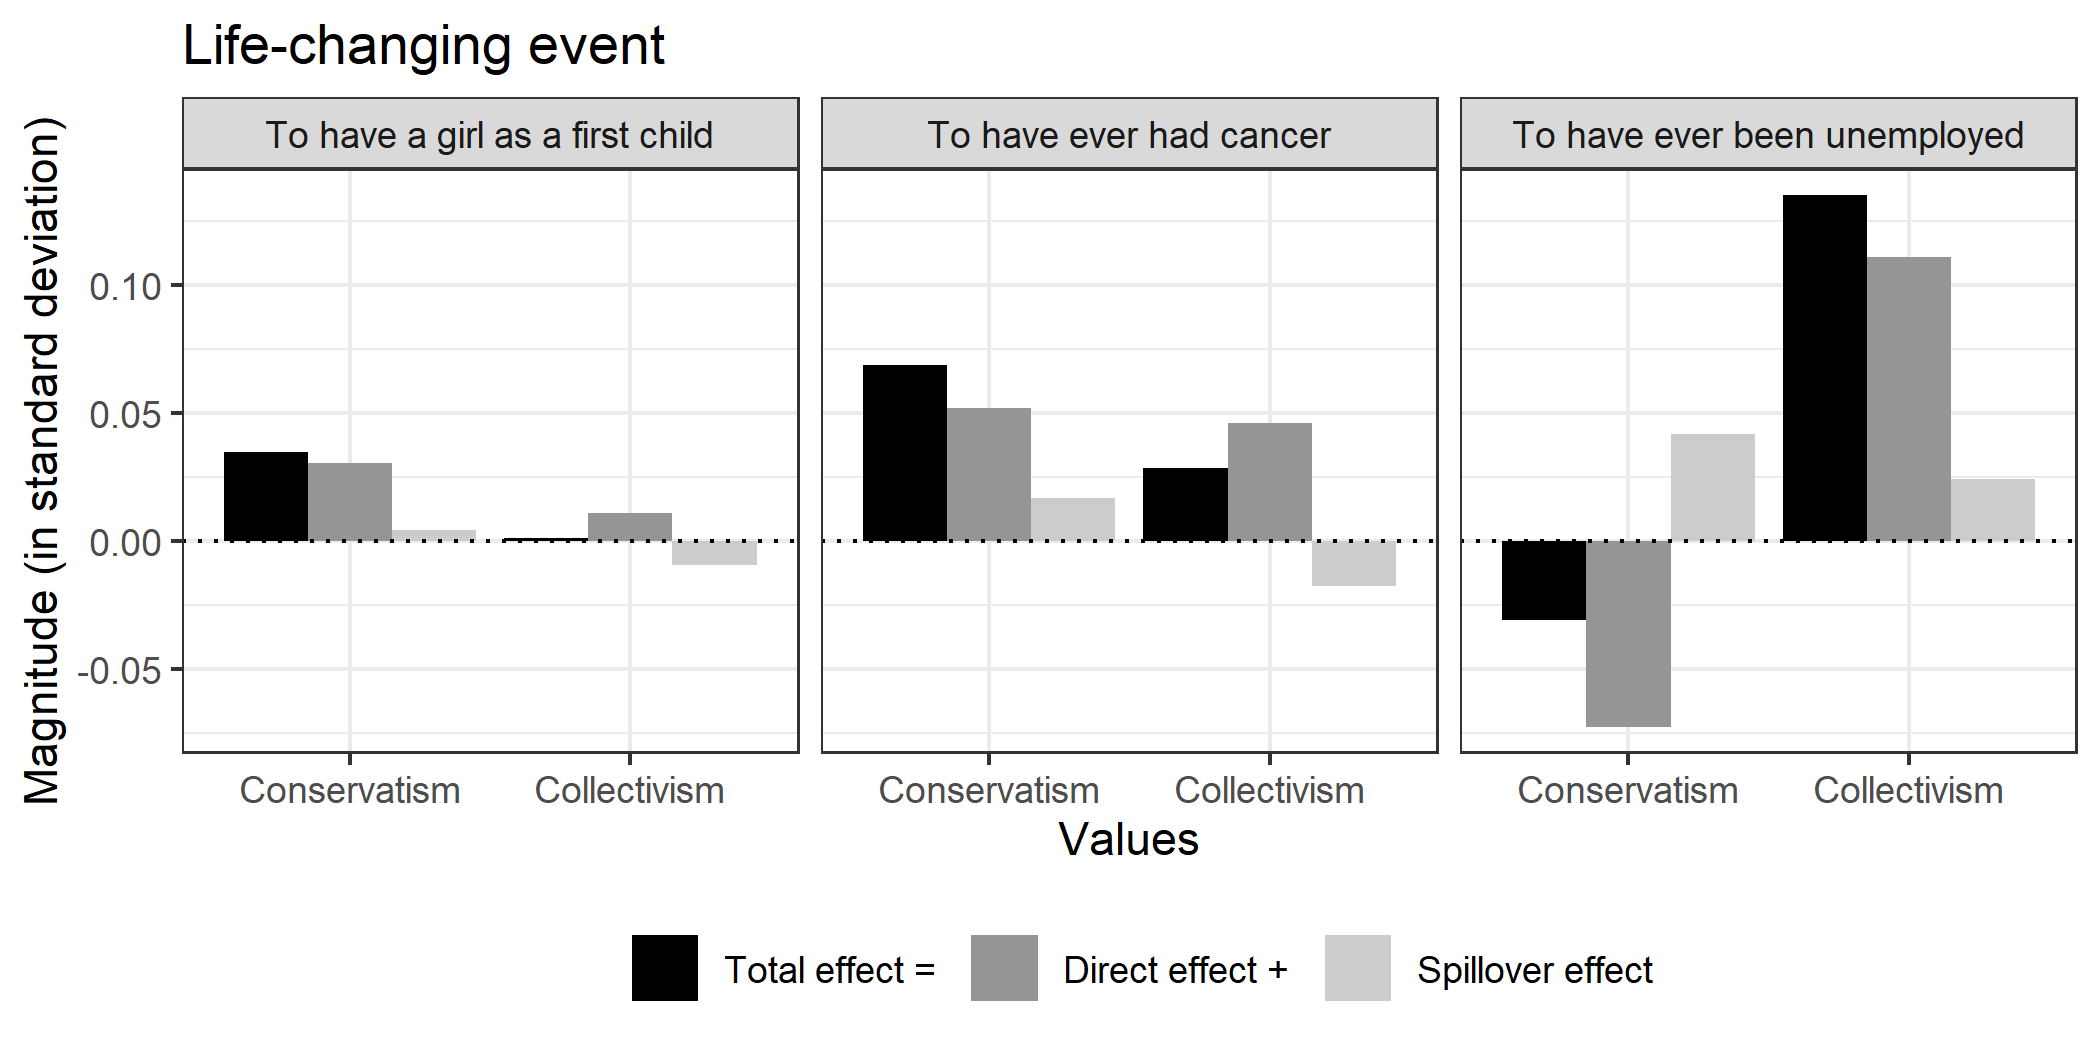
\includegraphics[width=\linewidth]{chap3/graphic/decomp-v5-base.png}
    \hrulefill
	\vspace{-3em}
	\justify\singlespacing\footnotesize{\textit{Notes:} This figure presents the decomposition of the total effect of each life-changing event on both values, Conservatism and Collectivism. The magnitude of effects is expressed in standard deviation. Decompositions are respectively derived from tables \ref{chap3-tab:decomp-GF}, \ref{chap3-tab:decomp-GC} and \ref{chap3-tab:decomp-BU}.}
\end{figure}
Having a girl as a first child directly increases conservative values by 0.03 standard deviation and collectivism by 0.01 standard deviation. Due to the consistency of values, about 14\% of the increase in conservatism is amplified by the raise in collectivism that has a positive impact on conservatism. Meanwhile, the increase in conservatism totally offsets the increase in collectivism, leading to a total effect that is negative although close to zero. Thus, due to the consistency of values and therefore the offsetting effect, collectivism does not increase when an individual gets a girl as a first child rather than a boy, while conservative values do increase. % This reconcile what we have seen in raw reg

Looking at heterogeneity across parents that are affected by this life event delivers two results (see figure \ref{chap3-fig:sem-decomp-v5-GFGender} and \ref{chap3-fig:sem-decomp-v5-GFEduc} in appendix \ref{chap3-estimates}). 
% Split by parents gender
First, for both, mothers and fathers, the direct effects go in the same direction---conservatism and collectivism---but they are more pronounced for mothers. For fathers, the negative spillover effect on collectivism offsets the positive information shock which leads to an increase in individualism. 
% Split by parents education
Second, splitting parents according to their education level shows that those with secondary education are the most affected. The effect of having a girl as a first child on tertiary-educated parents generates more progressive values which is consistent with \citet{Washington2008Female} results showing that congresspersons, hence, mostly highly educated men, become more progressive in their voting after having a daughter.

% HAVING EVER HAD CANCER
Having ever had cancer directly increases both conservatism and collectivism by 0.05 standard deviation. Due to values consistency, the increase in collectivism also increases conservative values through the spillover effect by 0.02 standard deviation, which represents almost a fourth of the total effect on conservatism. Meanwhile, part of the effect on collectivism is offset by the spillover effect of the life event through conservatism. As conservatism raises, it also decreases collectivism by 0.02 standard deviation which corresponds to 38\% of the direct effect. Thus, without the consistency of values, the increase in collectivism would have been 38\% much larger.

One may be concerned by the NCDS58 cohort at age 50 as they are likely to anticipate sickness, thus, changing their values. Excluding the NCDS58 cohort at age 50 provides very similar results with respect to the full sample, whereas considering exclusively this cohort at that age shows that the direct effect on conservatism is four times larger with respect to the baseline specification (see figure \ref{chap3-fig:sem-decomp-v5-GCNCDS58} in appendix \ref{chap3-estimates}). Interestingly, the direct effect on collectivism is much closer to zero. Thus, those who have had cancer at age 50 are not different from those who have not had one. Such an effect may be due to the anticipation of the sickness of the whole cohort at that age as they will rely more on others, hence, they increase their collectivist values. Nonetheless, the total effect on collectivism is positive---about 0.1 standard deviation---which is mostly due to the positive spillover effect on collectivism.
I also provide these estimates by focusing only on individuals who have never had cancer in the previous period (see figure \ref{chap3-fig:sem-decomp-v5-GCNever} in appendix \ref{chap3-estimates}). Although the direct effect on collectivism is larger, qualitative results hold.

% HAVING EVER BEEN UNEMPLOYED
Focusing on the third panel, those who have ever been unemployed experience a direct decline in conservatism, i.e. an increase in progressivism, by 0.07 standard deviation and a direct increase in collectivism by 0.11 standard deviation. The spillover effect of the decline in conservatism increases collectivist values by 0.02 standard deviation. Thus, collectivism raises by 22\% due to the spillover effect. Meanwhile, the increase in collectivism generates a positive spillover effect on conservative values which offsets half of the direct raise in progressivism. As a result, the increase in conservatism is dampened by the spillover effect whereas collectivism increases substantively.\footnote{In the extension of the theoretical framework in appendix \ref{chap3-model2}, I show that there is a bias when measuring the effect of an endogenous life event---such as unemployment---on values and I derive its expression. The bias does not affect the relative shares of the total effect that are due to the direct and spillover effects, nor the sign of the latter. However, the bias may affect the magnitude of the effect. In an extreme case of endogeneity of unemployment to values, the magnitudes have to be multiplied by a factor of 2/5, whereas feasible scenarii are likely to lie with a scale factor ranging from 1 (no endogeneity) to 2/3.}

One may be concerned by the current employment status that would be the driving factor for the effect of having ever been unemployed on values. I estimate the SEM using two subsamples (see figure \ref{chap3-fig:sem-decomp-v5-BUActivity} in appendix \ref{chap3-estimates}). First, I remove unemployed individuals at the time of the interview, then, I remove those out-of-work (unemployed and inactive). Both estimates do not differ with respect to the full sample one.

\subsection{Spillover effects' dynamics}

The intensity of inter-dependence between values drives the magnitude of the spillover effects of life events on values. In the SEM, the matrix $\Gamma$ captures the relation between values within the structural form. Once we consider the estimated reduced form for the decomposition, the spillover effects appear through $\Gamma^{-1}$. For instance, in the case of the girl-first life event, the $\Gamma$ matrix corresponds to
\begin{equation*}
    \Gamma = \begin{pmatrix}1 & 0.39 \\ -0.31 & 1\end{pmatrix} \implies \Gamma^{-1} = \begin{pmatrix}0.89 & -0.35 \\ 0.28 & 0.89\end{pmatrix}.
\end{equation*}
For both other life events, the coefficients in the matrices $\Gamma$ are very close to these ones which indicates that spillover effects do not depend on life events but are rather inherent.%
\footnote{See tables \ref{chap3-tab:reg-v5-sem-GC-stage12} and \ref{chap3-tab:reg-v5-sem-BU-stage12} in the appendix from which the $\Gamma$ matrix can be derived. For the got-cancer life event, $\Gamma = \begin{pmatrix}1 & 0.37 \\ -0.34 & 1\end{pmatrix}$. For the been-unmployed life event, $\Gamma = \begin{pmatrix}1 & 0.37 \\ -0.33 & 1\end{pmatrix}$.}
Thus, the effect of the life event $Z$ on values is derived from the matrix product of $\Theta = \begin{pmatrix} \theta_{Cons} & \theta_{Coll} \end{pmatrix}$ and the propagation matrix $\Gamma^{-1}$ that accounts for direct and spillover effects.

Considering the effect of the life event $Z$ on both values as a homogeneous system of first-order linear differential equations leads to
\begin{align*}
    x^\prime &= 0.89 x + 0.28 y,\\
    y^\prime &= -0.35 x + 0.89 y,
\end{align*}
where $x$ and $y$ are the magnitudes of both information shocks from $\Theta$, whereas $x^\prime$ and $y^\prime$ correspond to the net effects on values from $\Phi$. Solving this system leads to complex eigenvalues with positive real parts. This is due to the fact that, in $\Gamma$, the coefficients on the diagonal are equal to one and both off-diagonal coefficients have opposite signs. 

Figure \ref{chap3-fig:phase-plane} illustrates the phase plane of this system.
\begin{figure}[!tb]
    \centering
    \caption{Dynamics between values}
    \label{chap3-fig:phase-plane}
    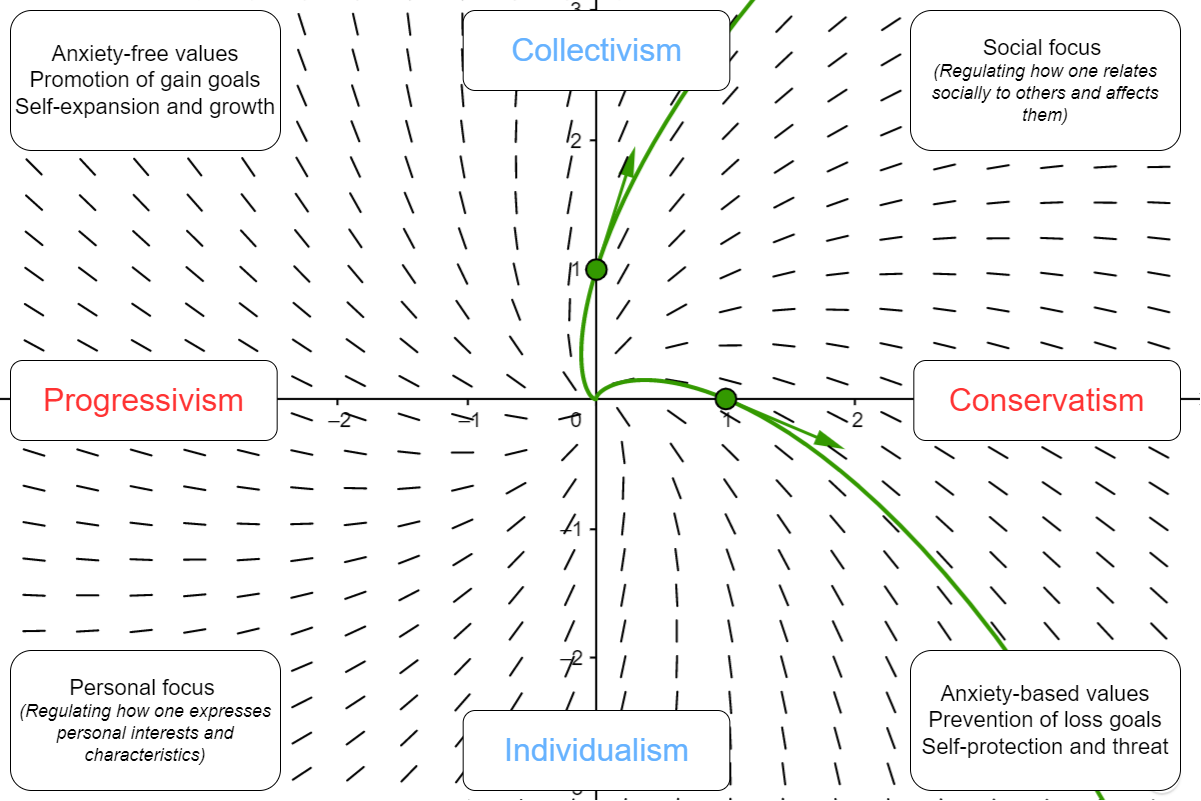
\includegraphics[width=\linewidth]{chap3/graphic/sys-diff-eq-plus.png}
	\vspace{-3em}
	\justify\singlespacing\footnotesize{\textit{Notes:} This figure presents the phase plane of the homogeneous system of first-order linear differential equations that describes the relationship between conservatism (versus progressivism) and collectivism (versus individualism) values. Green arrows decompose the direct effect and the indirect effect, i.e. spillover effect, due to a one standard deviation increase in each value.}
\end{figure}
Green dots are set to 1 on both axis, thus, the green arrows describe what happens for a one standard deviation increase on either the x-axis or the y-axis, i.e. in conservatism or in collectivism. An increase in conservatism has a negative spillover effect on collectivism, while an increase in collectivism has a positive spillover effect on conservatism. Thus, the relationship between values is \textit{not reciprocal} because of the spiral pattern in the system of first-order linear differential equations that is derived from the propagation matrix $\Gamma$.

Social psychology literature provides dynamic principles that shed light on the spiral pattern. Those principles correspond to the dynamic underpinnings of changes in values and correspond to the four corners of the figure (see \citealt{Schwartz2012Overview} for more details). For instance, any simultaneous increase in both conservatism and collectivism values, hence toward the top-right corner, refers to a raise in \textit{social focus}, i.e. preferring to live within a community and reinforcing the stability, tradition, and conformity to that community. Conversely, a decrease in those two values, hence toward the bottom-left corner, correspond to a raise in \textit{personal focus}, i.e. preferring to focus on self and not being constrained by rules. Looking at the two other corners, when individualism increases along with conservatism, hence toward the bottom-right corner, this refers to changes in values that help to deal with anxiety and the fear of loss goals, thus, they are self-protective values. Conversely, the top-left corner corresponds to self-expansive and anxiety-free based values.

Examining the spiral pattern of spillover effects through the lens of the dynamic underpinnings of value changes from social psychology provides several keys to understanding how life events affect individuals' values in figure \ref{chap3-fig:sem-decomp-v5-base}.
First, the initial increase in conservatism for both girl-first and got-cancer life events generates a spillover in individualism as those two life events are associated with anxiety, hence, self-protective values. Meanwhile, the initial raise of collectivist values reinforces the increase in conservatism by generating a positive spillover as it triggers a rise in social focus, i.e. relying more on the community and its rules.
For the been-unemployed life event, the initial increase in progressivism characterizes an increase in anxiety-free values as the fear of unemployed is not relevant anymore compared to those who have never been unemployed, hence, preventing themselves from losses. This raise in anxiety-free values has a positive impact on collectivism. The direct effect on collectivism is positive as the individual had relied more on the community since she had been unemployed, thus, this increases the social focus, hence conservative values.